\graphicspath{{content/11-reference/images/}}

\chapter{Référence}

\section{Utilisation de Rsnap}

\subsection{Créer une mission}
\begin{figure}[H]
  \begin{center}
    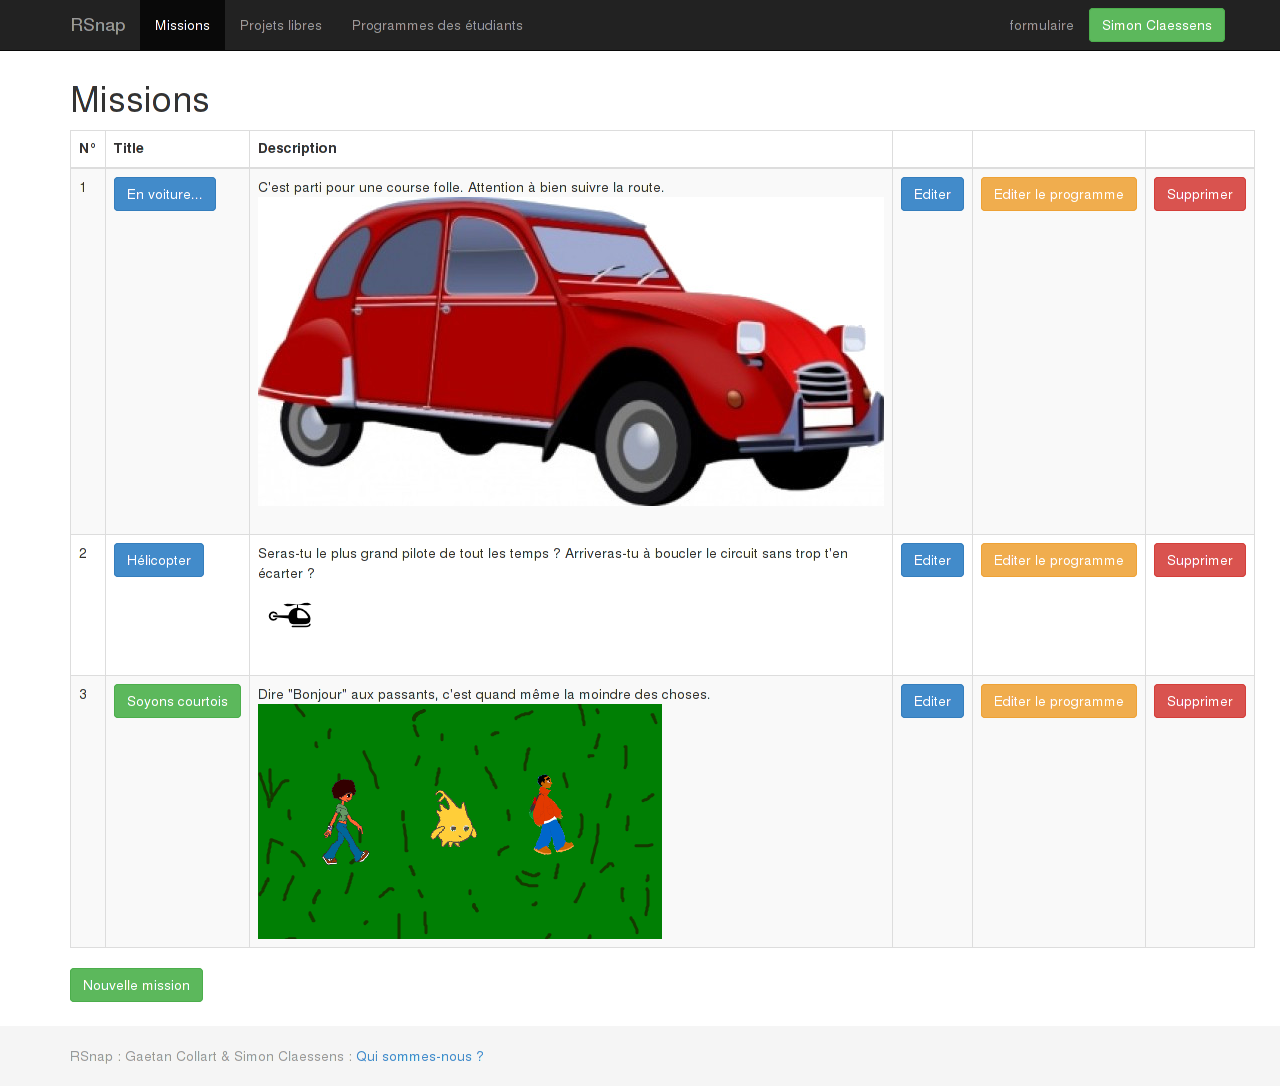
\includegraphics[width=\textwidth]{creer-mission-1}
    \caption{Page des missions}
    \label{fig:creer-mission-1}
  \end{center}
\end{figure}
\begin{figure}[H]
  \begin{center}
    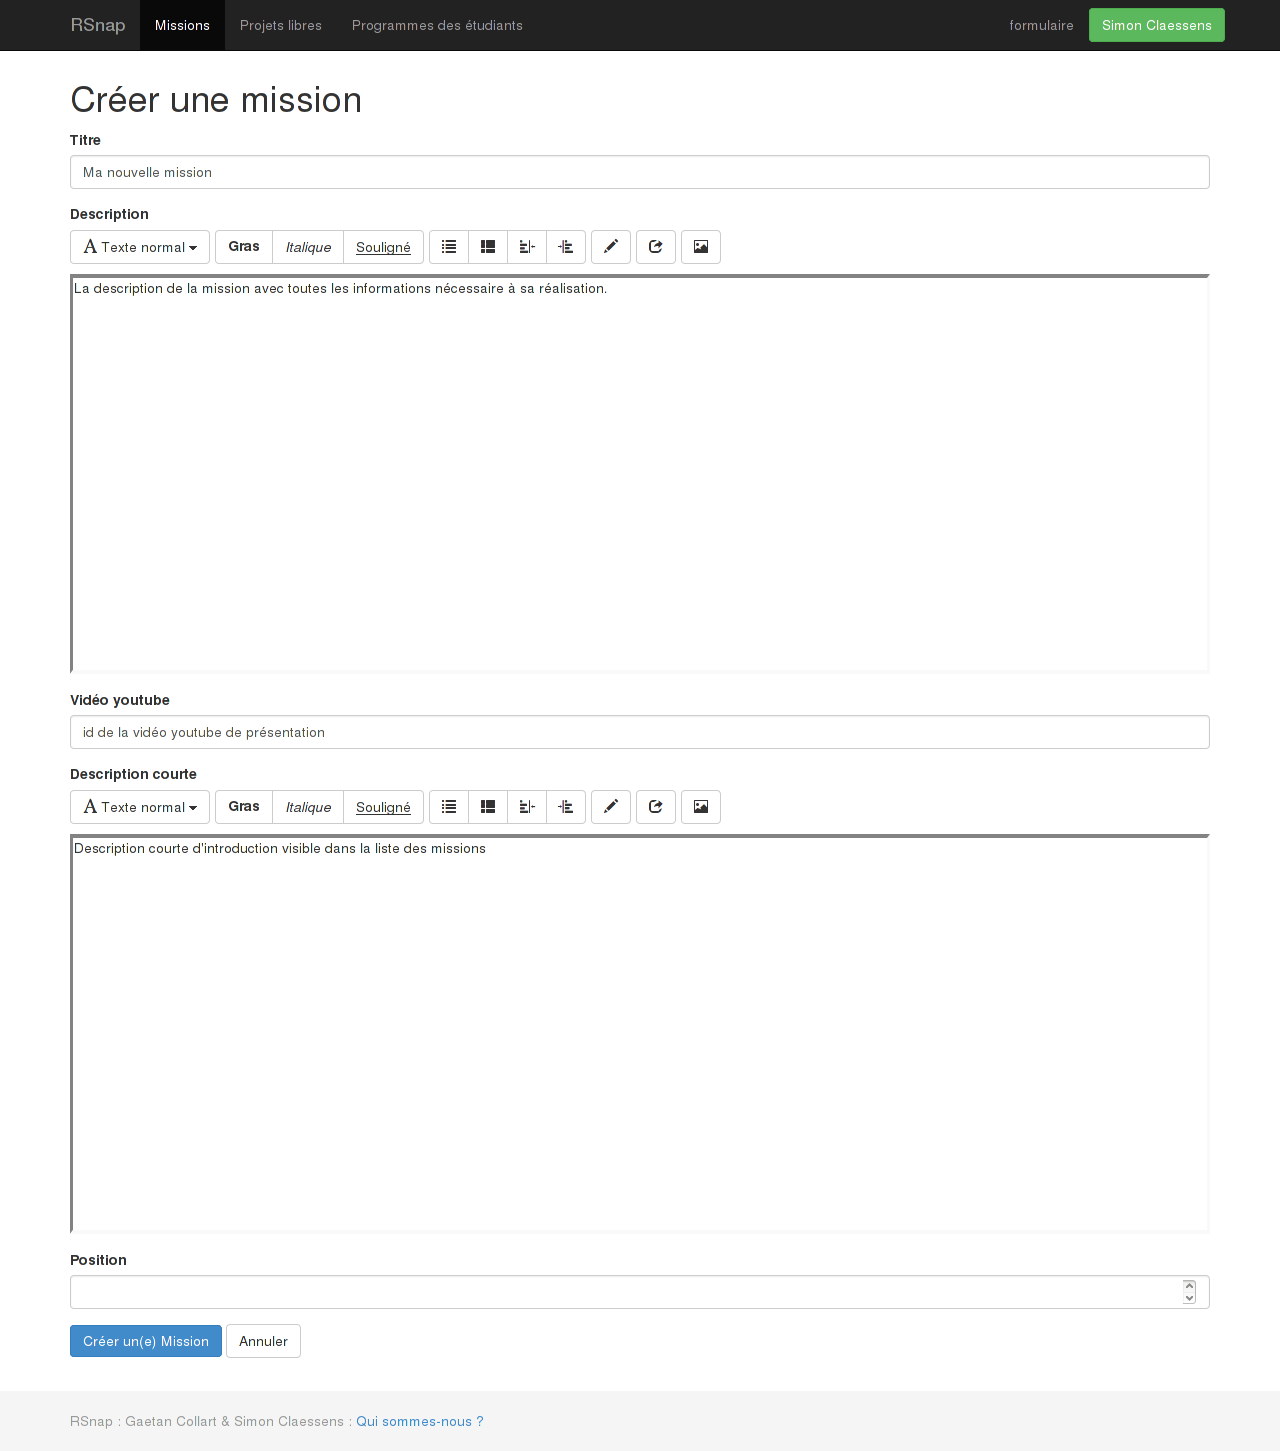
\includegraphics[width=\textwidth]{creer-mission-2}
    \caption{Création des informations de la mission}
    \label{fig:creer-mission-2}
  \end{center}
\end{figure}
\begin{figure}[H]
  \begin{center}
    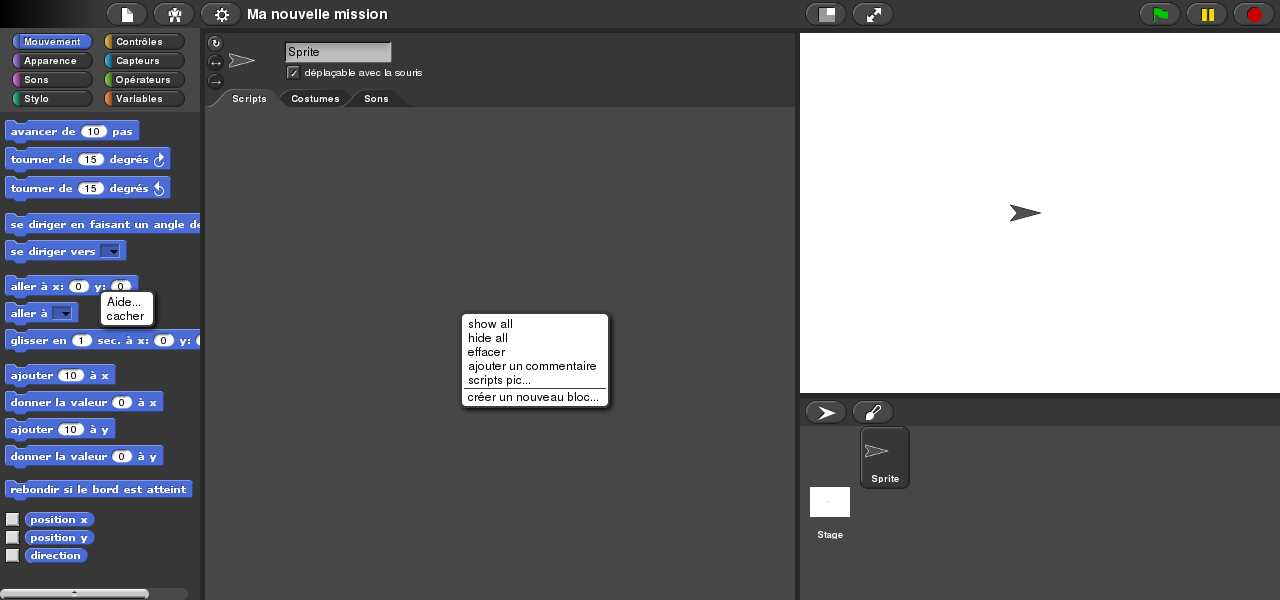
\includegraphics[width=\textwidth]{creer-mission-3}
    \caption{Création du programme de la mission}
    \label{fig:creer-mission-3}
  \end{center}
\end{figure}

\FloatBarrier
\subsection{Ordonner les missions}
\begin{figure}[H]
  \begin{center}
    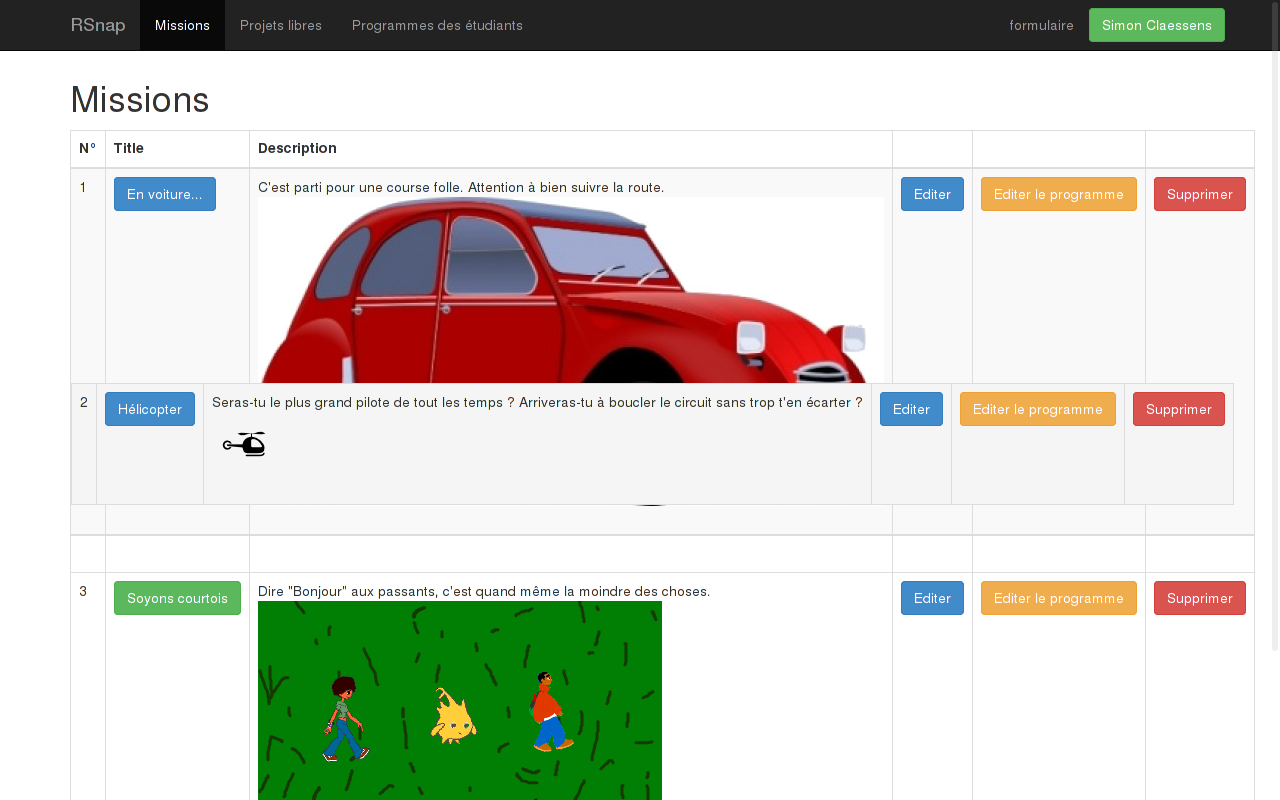
\includegraphics[width=\textwidth]{mission-order}
    \caption{Ordonner les missions}
    \label{fig:mission-order}
  \end{center}
\end{figure}

\FloatBarrier
\subsection{Corriger une mission}
\begin{figure}[H]
  \begin{center}
    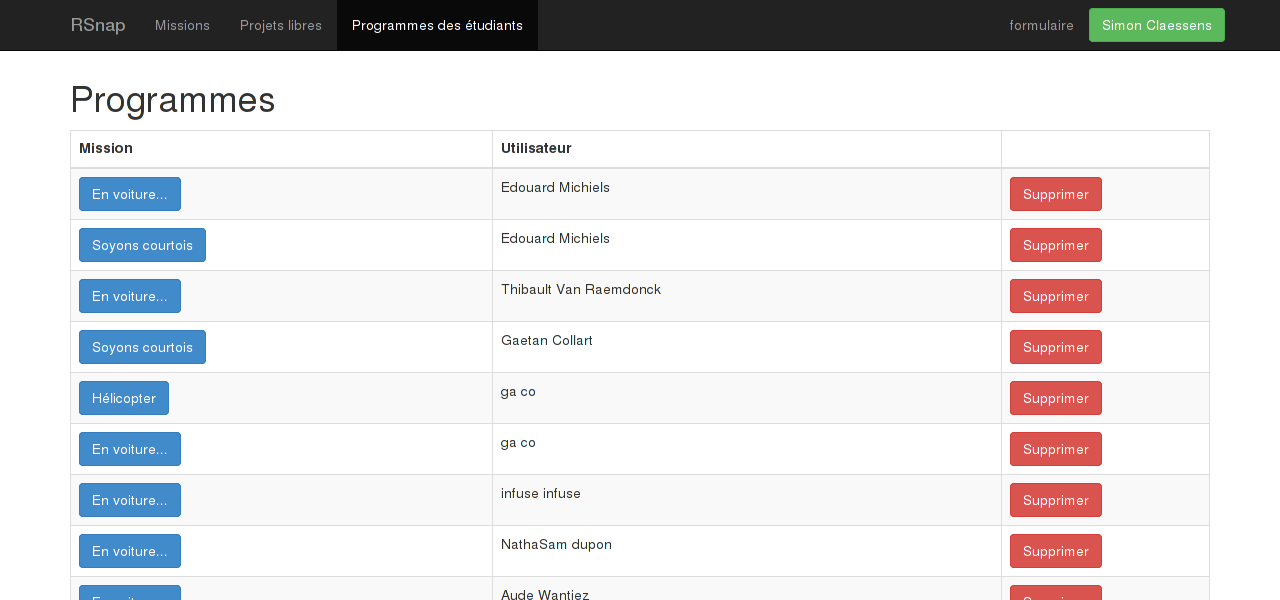
\includegraphics[width=\textwidth]{corriger-prog-1}
    \caption{Page des programmes des étudiants}
    \label{fig:corriger-prog-1}
  \end{center}
\end{figure}
\begin{figure}[H]
  \begin{center}
    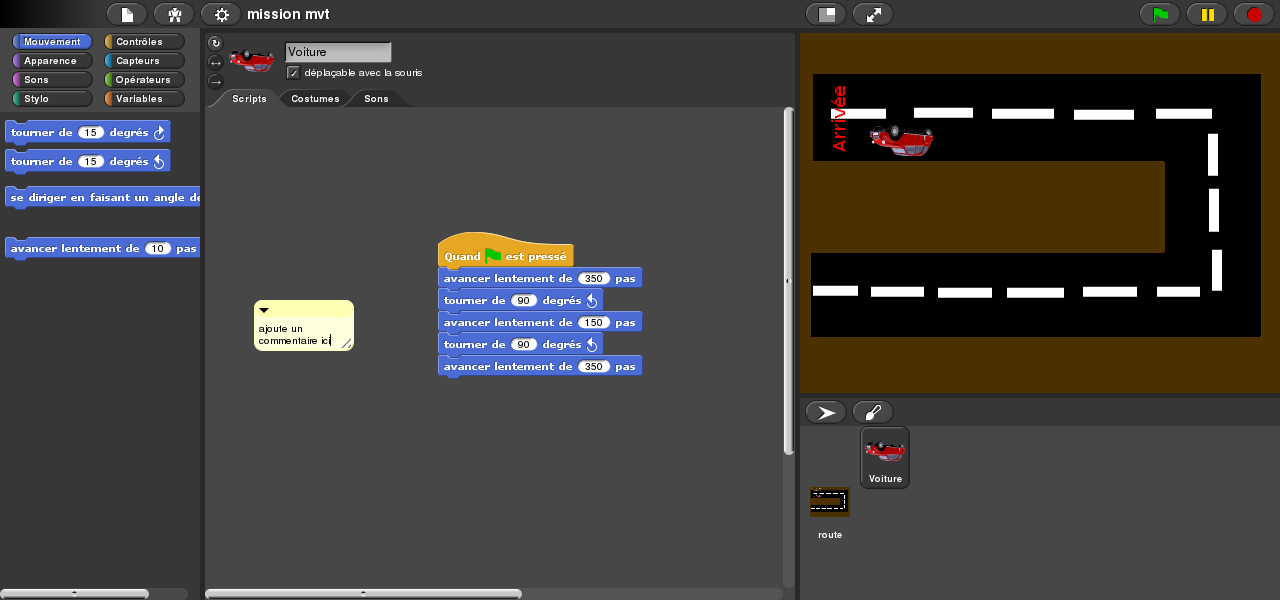
\includegraphics[width=\textwidth]{corriger-prog-2}
    \caption{Correction du programme}
    \label{fig:corriger-prog-2}
  \end{center}
\end{figure}

\FloatBarrier
\subsection{Réaliser une mission}
\begin{figure}[H]
  \begin{center}
    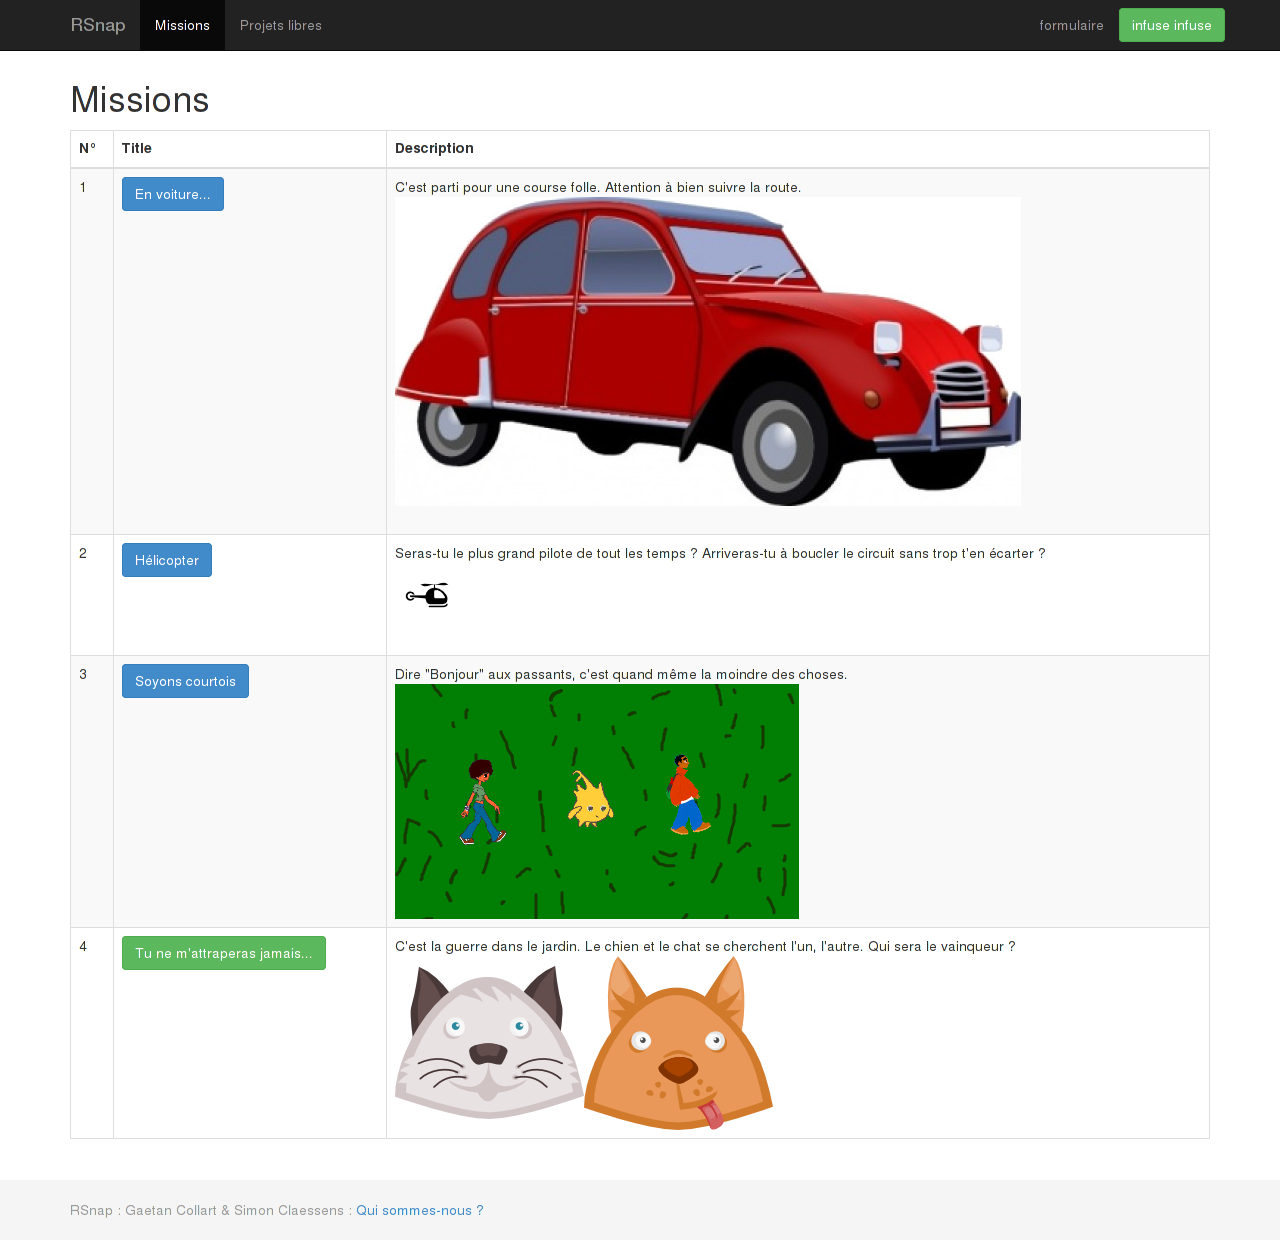
\includegraphics[width=\textwidth]{realiser-mission-1}
    \caption{Page des missions}
    \label{fig:realiser-mission-1}
  \end{center}
\end{figure}
\begin{figure}[H]
  \begin{center}
    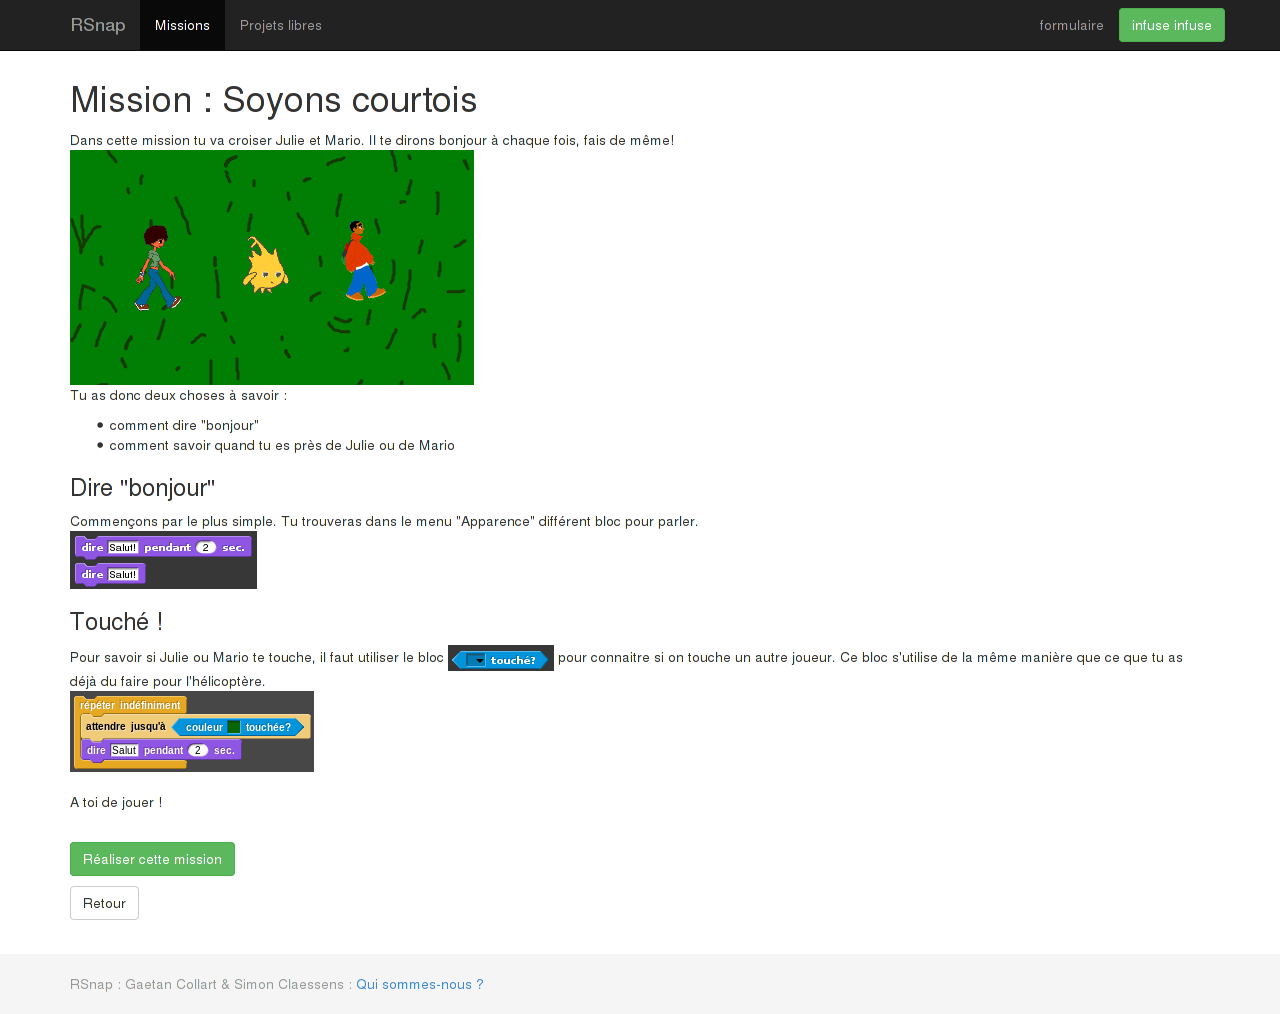
\includegraphics[width=\textwidth]{realiser-mission-2}
    \caption{Description de la mission}
    \label{fig:realiser-mission-2}
  \end{center}
\end{figure}
\begin{figure}[H]
  \begin{center}
    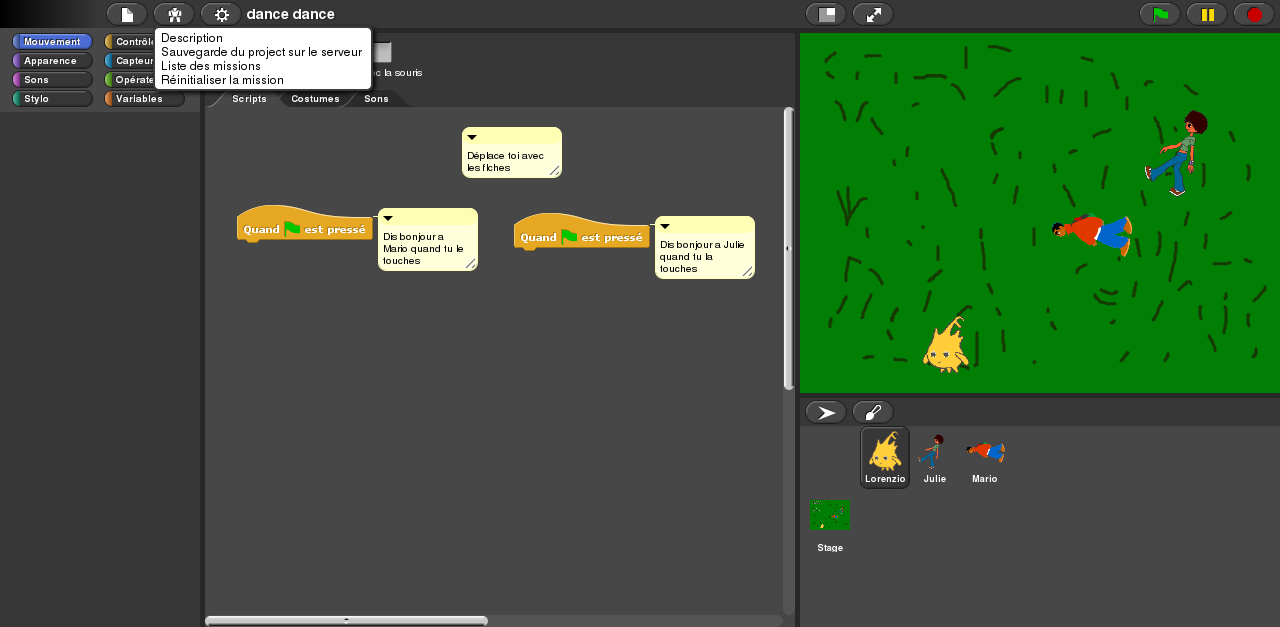
\includegraphics[width=\textwidth]{realiser-mission-3}
    \caption{Réalisation de la mission}
    \label{fig:realiser-mission-3}
  \end{center}
\end{figure}

\FloatBarrier
\subsection{Réaliser un projet libre}
\begin{figure}[H]
  \begin{center}
    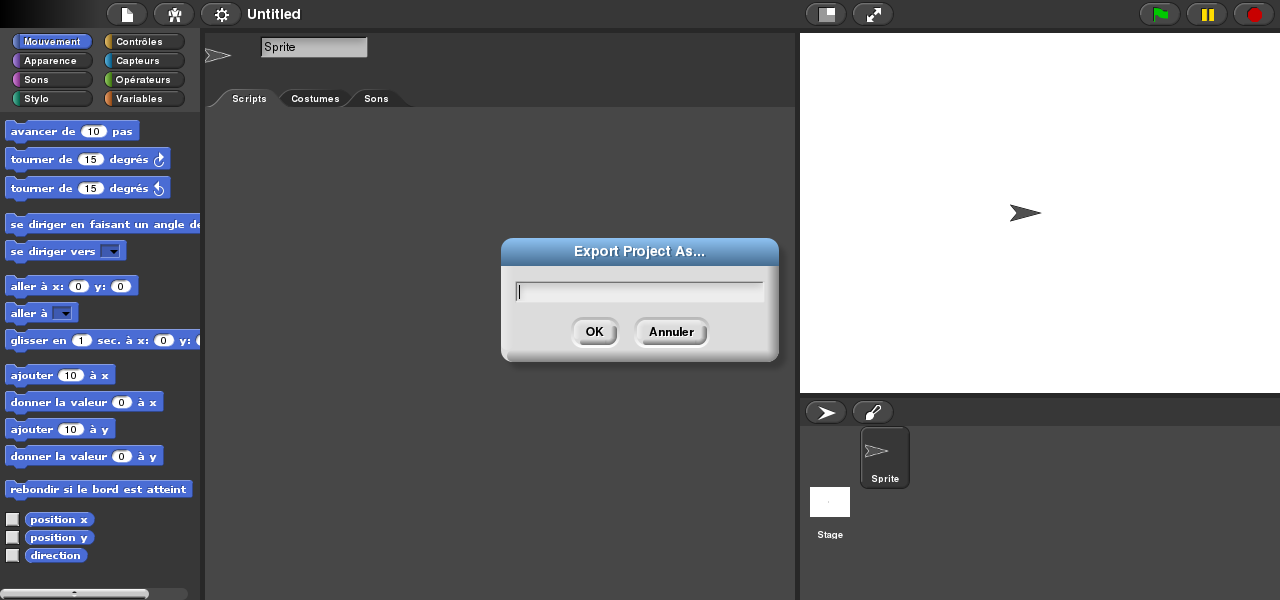
\includegraphics[width=\textwidth]{projet-1}
    \caption{Page des projets libres}
    \label{fig:projet-1}
  \end{center}
\end{figure}
\begin{figure}[H]
  \begin{center}
    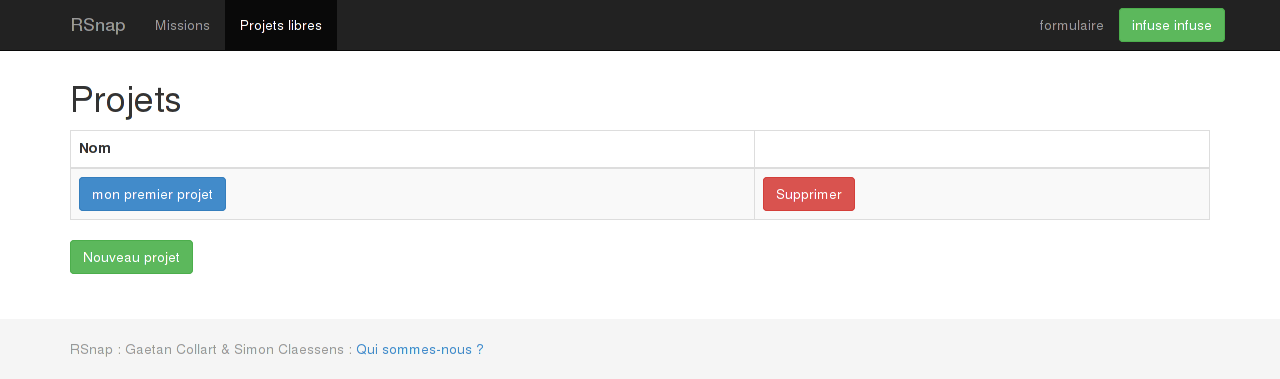
\includegraphics[width=\textwidth]{projet-2}
    \caption{Création du programme du projet libre}
    \label{fig:projet-2}
  \end{center}
\end{figure}

\FloatBarrier
\section{Réponses au formulaire des enfants}
\label{annex:forms}
\begin{table}
  \caption{Réponse aux questions d'ordre général}
  \label{tab:form-perso}

  \begin{center}
\rotatebox{270}{
    \begin{tabular}{|m{90pt}|m{65pt}|m{50pt}|m{55pt}|m{55pt}|m{65pt}|m{85pt}|}
\hline
Je suis à ...&Je suis en ...&Je savais utiliser un ordinateur avant de venir ?&Je sais mieux utiliser un ordinateur maintenant ?&Je savais ce qu'était la programmation avant de venir ?&Je comprend mieux ce qu'est la programmation maintenant ?&J'ai encore des choses à vous dire.\\
\hline
\hline
Collège Cardinal Mercier&1e secondaire&3&3&4&3&\\
Collège Saint Joseph &1e secondaire&3&4&2&4&\\
Collège Saint-Joseph Chimay&1e secondaire&3&1&3&3&nan\\
college st joseph chimay&1e secondaire&2&2&1&3&\\
au college saint josephe de chimay&1e secondaire&4&4&1&4&\\
college saint joseph&1e secondaire&2&3&1&3&\\
collège saint joseph à chimay&1e secondaire&3&3&1&4&bon courrage pour votre fin d'année!!! félicitation\\
collège st Joseph chimay&1e secondaire&2&3&2&3&\\
Saint Joseph Chimay&1e secondaire&3&3&1&4&\\
Collège St Joseph  &1e secondaire&2&3&1&3&c etais cool\\
\hline
    \end{tabular}
}
  \end{center}
\end{table}

\begin{table}
  \caption{Réponse aux questions d'ordre général (suite)}
  \label{tab:form-perso2}

  \begin{center}
\rotatebox{270}{
    \begin{tabular}{|m{60pt}|m{65pt}|m{50pt}|m{55pt}|m{55pt}|m{65pt}|m{115pt}|}
\hline
Je suis à ...&Je suis en ...&Je savais utiliser un ordinateur avant de venir ?&Je sais mieux utiliser un ordinateur maintenant ?&Je savais ce qu'était la programmation avant de venir ?&Je comprend mieux ce qu'est la programmation maintenant ?&J'ai encore des choses à vous dire.\\
\hline
\hline
Collège St Joseph  &1e secondaire&4&4&0&0&\\
collège saint joseph&1e secondaire&4&1&1&3&amusant, des missions plus faciles que les autres, beaucoup de réfléxions.\\
college saint joseph&1e secondaire&4&1&2&4&\\
st-joseph&1e secondaire&4&4&1&4&c'etais trop cool on ces bien amuser merci !!!!!!!!!!!\\
Collège Saint Joseph &1e secondaire&4&1&4&1&\\
college saint joseph 1c8&1e secondaire&4&3&2&4&non\\
Chimay&1e secondaire&3&2&1&2&que c'était en partit quand même bien malgré le soucis\\
\hline
    \end{tabular}
}
  \end{center}
\end{table}

\begin{table}
  \caption{Réponse aux questions d'ordre général (suite 2)}
  \label{tab:form-perso3}

  \begin{center}
\rotatebox{270}{
    \begin{tabular}{|m{75pt}|m{65pt}|m{50pt}|m{55pt}|m{55pt}|m{65pt}|m{100pt}|}
\hline
Je suis à ...&Je suis en ...&Je savais utiliser un ordinateur avant de venir ?&Je sais mieux utiliser un ordinateur maintenant ?&Je savais ce qu'était la programmation avant de venir ?&Je comprend mieux ce qu'est la programmation maintenant ?&J'ai encore des choses à vous dire.\\
\hline
\hline
collège saint joseph à chimay&1e secondaire&2&2&1&4&\\
collège st Joseph chimay&1e secondaire&4&1&2&3&\\
au college saint josephe de chimay&1e secondaire&2&1&1&1&\\
st marie &6e primaire&4&4&0&4&\\
ecole st marie bousval&6e primaire&3&3&1&4&un peu plus de mission dans ce genre et des mission un peu plus compliquer pour les plus grand et des plus facile pour les plus petit\\
sainte marie&6e primaire&4&1&3&3&\\
rendeux&6e primaire&2&2&2&3&\\
\hline
    \end{tabular}
}
  \end{center}
\end{table}

\begin{table}
  \caption{Réponse aux questions d'ordre général (suite 3)}
  \label{tab:form-perso4}

  \begin{center}
\rotatebox{270}{
    \begin{tabular}{|m{70pt}|m{55pt}|m{50pt}|m{55pt}|m{55pt}|m{65pt}|m{115pt}|}
\hline
Je suis à ...&Je suis en ...&Je savais utiliser un ordinateur avant de venir ?&Je sais mieux utiliser un ordinateur maintenant ?&Je savais ce qu'était la programmation avant de venir ?&Je comprend mieux ce qu'est la programmation maintenant ?&J'ai encore des choses à vous dire.\\
\hline
\hline
ecole Ste Marie&6e primaire&4&1&1&4&PLUS VITE CET BIIIIIIIIIIIIP D'ORDINATEUR!!!\\
Sainte-Marie&6e primaire&4&2&3&4&non juste les bug\\
école St-Marie&6e primaire&4&4&1&3&\\
Ecole Sainte Marie&6e primaire&2&4&1&3&s etais trop COOL et on sais bien amusé\\
Collège du Biéreau&6e primaire&4&1&4&4&\\
aro&6e primaire&3&2&1&3&\\
aro&6e primaire&4&4&1&4&\\
aro&6e primaire&4&1&0&4&\\
 aro paul delvaux ottignies&6e primaire&2&3&1&1&c est trop dur mais sava\\
 A.R.O.&6e primaire&4&1&3&4&\\
ARO&6e primaire&4&2&3&3&\\
athenée royal paul delvaux d'ottignies&6e primaire&4&1&2&4&\\
\hline
    \end{tabular}
}
  \end{center}
\end{table}


\begin{table}
  \caption{Réponse relative à la mission "En voiture"}
  \label{tab:form-voiture}

  \begin{center}
\rotatebox{270}{
    \begin{tabular}{|m{50pt}|m{75pt}|m{75pt}|m{75pt}|m{215pt}|}
\hline
J'ai aimé réaliser cette mission ?&Avec les explications données et le texte décrivant la mission, j'ai compris le but de la mission ?&Avec les explications données et le texte décrivant la mission, j'ai su par où commencer ?&Avec les explications données et le texte décrivant la mission, j'ai réalisé la mission ?&J'ai des remarques à transmettre.\\
\hline
\hline
4&4&3&4&\\
3&2&4&4&\\
4&3&4&4&C'était fort bien sympathique :) On aimerait recommencer un jour ! \\
2&1&1&4&j ai pas tres bien compris les donnees sur le cote de l ecran \\
4&4&3&4&\\
4&4&4&4&rien est a ameliorer c'etait génial!!!\\
2&2&2&3&une meilleur explication aurait été plus émable en tout cas...\\
3&3&4&4&J ai bien aimé la mission de la voiture \\
4&4&3&4&j ai tous aime :),je n ai rien détesté,tous,rien\\
4&3&4&3&c etais cool j ai bien aimé utiliser les bloques et faire avancer la voiture et surtout quand on a réussit on etait content bref  on a bien aimer merci :)\\
4&3&3&3&\\
4&4&2&3&\\
4&4&3&4&\\
\hline
    \end{tabular}
}
  \end{center}
\end{table}

\begin{table}
  \caption{Réponse relative à la mission "En voiture" (suite)}
  \label{tab:form-voiture2}

  \begin{center}
\rotatebox{270}{
    \begin{tabular}{|m{50pt}|m{75pt}|m{75pt}|m{75pt}|m{215pt}|}
\hline
J'ai aimé réaliser cette mission ?&Avec les explications données et le texte décrivant la mission, j'ai compris le but de la mission ?&Avec les explications données et le texte décrivant la mission, j'ai su par où commencer ?&Avec les explications données et le texte décrivant la mission, j'ai réalisé la mission ?&J'ai des remarques à transmettre.\\
\hline
\hline
4&3&3&3&au depart on comprenait pas trop mais mantenant ces beaucoup plus facile\\
4&4&4&4&j ai tout aimer ;) ;) ;)\\
4&4&4&3&\\
3&3&3&4&C'était bien on s'est bien amusée mais il y a des missions qu'on n'a pas trop aimé car on ne savait pas ce qu'il fallait faire\\
4&2&1&3&LA LOGIQUE ÉTAIS BIEN MAI SELLA ÉTAIT TRÈS TRÈS DURE NOUS AVONS pas SU RÉPONDRE SANS LAIDE DES ACOMPAGNIATEUR\\
2&3&3&3&nous avons trouver sa marrant , au début c était dur mais a la fin sa allait c est bien expliquer \\
3&2&1&2&je n ai rien a dire \\
4&4&4&4&j'ai adorée\\
4&3&3&3&la m!ission etait bien amusante et chouette a realiser\\
3&4&4&3&les lags etaient genant\\
\hline
    \end{tabular}
}
  \end{center}
\end{table}

\begin{table}
  \caption{Réponse relative à la mission "En voiture" (suite 2)}
  \label{tab:form-voiture3}

  \begin{center}
\rotatebox{270}{
    \begin{tabular}{|m{50pt}|m{75pt}|m{75pt}|m{75pt}|m{215pt}|}
\hline
J'ai aimé réaliser cette mission ?&Avec les explications données et le texte décrivant la mission, j'ai compris le but de la mission ?&Avec les explications données et le texte décrivant la mission, j'ai su par où commencer ?&Avec les explications données et le texte décrivant la mission, j'ai réalisé la mission ?&J'ai des remarques à transmettre.\\
\hline
\hline
3&4&4&3&\\
4&4&4&3&la rapidité de l'ordinateur\\
4&4&4&2&des bug\\
4&3&4&4&nous avons aimé parce que se n'étais pas trop difficile et que nous nous sommes bien amusée\\
3&1&2&3&votre ordinateur est tres tres lent et animation etais cool\\
4&4&4&4&\\
4&3&3&3&\\
4&4&4&4&\\
4&4&4&4&\\
2&1&3&3&c estait bien sauf quand sa fesait boum\\
4&3&3&4&Très chouette on a bien rigolé \\
3&2&1&3&Ce projet est une très bonne idée mais les explications n'etaient pas claires et programme buggait\\
3&3&1&1&on a eu quelque difficultée a la premiere mission mais apres on\\
\hline
    \end{tabular}
}
  \end{center}
\end{table}

\begin{table}
  \caption{Réponse relative à la mission "Hélicoptère"}
  \label{tab:form-helico}

  \begin{center}
\rotatebox{270}{
    \begin{tabular}{|m{50pt}|m{75pt}|m{75pt}|m{75pt}|m{215pt}|}
\hline
J'ai aimé réaliser cette mission ?&Avec les explications données et le texte décrivant la mission, j'ai compris le but de la mission ?&Avec les explications données et le texte décrivant la mission, j'ai su par où commencer ?&Avec les explications données et le texte décrivant la mission, j'ai réalisé la mission ?&J'ai des remarques à transmettre.\\
\hline
\hline
3&3&4&3&\\
4&3&4&3&\\
3&2&4&3&Rien à dire :D\\
2&3&2&1&apres qu on nous ai expliquer nous avons compris\\
4&3&2&4&ca fait boum quand on touche la ligne vert\\
3&3&3&3&c'était bien mais je suis rester bloquer car je n'avais pas la bonne couleur :)\\
2&2&2&2&on ne nous a pas bien expliquer se qu il falait faire... a part ca rien n'a dire de grave\\
3&4&4&3&\\
4&4&4&4&J AI AIME\\
3&4&3&4&c etais cool\\ 
4&4&3&3&\\
4&2&1&4&\\
3&2&2&2&un peu compliquer a comprendre \\
4&3&2&3&\\
4&4&4&4&javate\\
3&3&4&3&\\
\hline
    \end{tabular}
}
  \end{center}
\end{table}

\begin{table}
  \caption{Réponse relative à la mission "Hélicoptère" (suite)}
  \label{tab:form-helico2}

  \begin{center}
\rotatebox{270}{
    \begin{tabular}{|m{50pt}|m{75pt}|m{75pt}|m{75pt}|m{215pt}|}
\hline
J'ai aimé réaliser cette mission ?&Avec les explications données et le texte décrivant la mission, j'ai compris le but de la mission ?&Avec les explications données et le texte décrivant la mission, j'ai su par où commencer ?&Avec les explications données et le texte décrivant la mission, j'ai réalisé la mission ?&J'ai des remarques à transmettre.\\
\hline
\hline
2&2&2&2&C'était compliqué on a du appeller quelqu'un\\
4&3&3&3&PLUTÔT COOL QUAND ON A COMPRIS MAI LES EXPLICATION NE TAIT pas FACILE A COMPRENDRE LA PREMIERES FOI \\
2&4&3&4&c’était sympas facile bien expliquer \\
1&2&1&2&\\
4&4&4&4&aucune remarque a dire parfait \\
4&4&4&4&on la fait que 1 fois et on a eu bon \\
4&4&4&3&il faut juste ameliorer la vitesse de l'helicoptere\\
4&3&4&4&\\
1&1&1&1&faites que se sois plus FACILE!!!!!!!!!!!!!!!!!!!!!!!!!!!!!!!!!!!!!!!!!!!!!!!!!\\
4&4&4&3&aussi bug\\
4&3&4&3&nous avons aimé car il y avait un peu de difficulté et on a bien rigoler \\
2&1&1&3&\\
4&4&4&4&\\
\hline
    \end{tabular}
}
  \end{center}
\end{table}

\begin{table}
  \caption{Réponse relative à la mission "Hélicoptère" (suite 2)}
  \label{tab:form-helico3}
  \begin{center}
\rotatebox{270}{
    \begin{tabular}{|m{50pt}|m{75pt}|m{75pt}|m{75pt}|m{215pt}|}
\hline
J'ai aimé réaliser cette mission ?&Avec les explications données et le texte décrivant la mission, j'ai compris le but de la mission ?&Avec les explications données et le texte décrivant la mission, j'ai su par où commencer ?&Avec les explications données et le texte décrivant la mission, j'ai réalisé la mission ?&J'ai des remarques à transmettre.\\
\hline
\hline
0&0&0&0&\\
1&1&1&1&\\
3&3&3&3&\\
0&0&0&0&\\
0&0&0&0&\\
2&1&1&1&\\
\hline
    \end{tabular}
}
  \end{center}
\end{table}



\begin{table}
  \caption{Réponse relative à la mission "Soyons courtois"}
  \label{tab:form-courtois}
  \begin{center}
\rotatebox{270}{
    \begin{tabular}{|m{50pt}|m{75pt}|m{75pt}|m{75pt}|m{215pt}|}
\hline
J'ai aimé réaliser cette mission ?&Avec les explications données et le texte décrivant la mission, j'ai compris le but de la mission ?&Avec les explications données et le texte décrivant la mission, j'ai su par où commencer ?&Avec les explications données et le texte décrivant la mission, j'ai réalisé la mission ?&J'ai des remarques à transmettre.\\
\hline
\hline
0&0&0&0&\\
4&4&4&4&\\
4&4&3&4&On a  bien aimé en général !\\
4&3&2&4&\\
4&2&3&4&\\
4&2&2&3&je n'avais pas trop compris mais des personnes m'on expliquer et j'ai compris :)\\
4&4&4&4&assez facile!!\\
1&3&3&3&\\
4&4&4&4&\\
3&4&3&4&c etais cool \\
4&2&2&2&\\
4&4&4&4&un peut trop facile \\
2&1&2&3&dur a comprendre\\
1&3&2&3&\\
4&4&4&4&setais trop fastoche\\
2&2&2&1&je n'ai pas comprit le but\\
3&3&3&3&On a eu un beug car ils ont pas mit parfait\\
2&1&1&1&JE NES RIEN A DIRE \\
\hline
    \end{tabular}
}
  \end{center}
\end{table}

\begin{table}
  \caption{Réponse relative à la mission "Soyons courtois" (suite)}
  \label{tab:form-courtois2}
  \begin{center}
\rotatebox{270}{
    \begin{tabular}{|m{50pt}|m{75pt}|m{75pt}|m{75pt}|m{215pt}|}
\hline
J'ai aimé réaliser cette mission ?&Avec les explications données et le texte décrivant la mission, j'ai compris le but de la mission ?&Avec les explications données et le texte décrivant la mission, j'ai su par où commencer ?&Avec les explications données et le texte décrivant la mission, j'ai réalisé la mission ?&J'ai des remarques à transmettre.\\
\hline
\hline
3&3&3&3&elle est cool mais un peu dur a comprendre au début \\
1&2&1&1&\\
0&0&0&0&\\
0&0&0&0&\\
0&0&0&0&\\
0&0&0&0&\\
0&0&0&0&\\
0&0&0&0&\\
0&0&0&0&\\
0&0&0&0&\\
0&0&0&0&\\
2&3&3&3&\\
3&3&3&3&\\
0&0&0&0&\\
1&1&1&1&c etais asser bien\\
2&2&0&3&\\
3&2&2&2&\\
2&3&4&4&c etait cool;l\\
\hline
    \end{tabular}
}
  \end{center}
\end{table}

\begin{table}
  \caption{Réponse relative à la mission "Tu ne m'attraperas pas"}
  \label{tab:form-attrapera}
  \begin{center}
\rotatebox{270}{
    \begin{tabular}{|m{50pt}|m{75pt}|m{75pt}|m{75pt}|m{215pt}|}
\hline
J'ai aimé réaliser cette mission ?&Avec les explications données et le texte décrivant la mission, j'ai compris le but de la mission ?&Avec les explications données et le texte décrivant la mission, j'ai su par où commencer ?&Avec les explications données et le texte décrivant la mission, j'ai réalisé la mission ?&J'ai des remarques à transmettre.\\
\hline
\hline
3&4&3&3&\\
4&4&3&4&\\
1&2&1&3&Un peu énervant :x\\
4&3&3&2&j ai beaucoups aimer\\
4&4&4&4&\\
3&2&2&2&j'ai pas trop compris et je n'ai même pas terminer mais sinojn c'était cool :) :)\\
3&3&3&3&on n'a pas sut terminées!!!\\
1&2&3&2&on c est beaucoup aidee\\
4&4&4&4&\\
3&4&3&4&c etais cool\\
4&4&4&4&\\
1&1&1&1&dûr à comprendre \\
3&2&3&3&\\
4&4&4&4&ces trop coollllllll!!!\\
4&4&4&4&trop trop trop trop trop trop trop trop trop trop trop                               cooooooooooooooooooooooooooooooooooool\\
1&1&1&1&je n'ai pas tout comprit .c'est compliqué\\
\hline
    \end{tabular}
}
  \end{center}
\end{table}

\begin{table}
  \caption{Réponse relative à la mission "Tu ne m'attraperas pas" (suite)}
  \label{tab:form-attrapera2}
  \begin{center}
\rotatebox{270}{
    \begin{tabular}{|m{50pt}|m{75pt}|m{75pt}|m{75pt}|m{215pt}|}
\hline
J'ai aimé réaliser cette mission ?&Avec les explications données et le texte décrivant la mission, j'ai compris le but de la mission ?&Avec les explications données et le texte décrivant la mission, j'ai su par où commencer ?&Avec les explications données et le texte décrivant la mission, j'ai réalisé la mission ?&J'ai des remarques à transmettre.\\
\hline
\hline
1&1&0&1&On a pas su la faire car quelqu'un est venu mais on a pas compris \\
1&1&1&1&SET AI HORRIBLEMENT DUR \\
3&3&3&3&cette mission est plutôt dur on ne comprend pas très bien mais c etait marrant surtout avec les personnage \\
1&1&1&1&\\
4&4&4&4&\\
3&3&3&3&\\
0&0&0&0&\\
0&0&0&0&\\
0&0&0&0&\\
0&0&0&0&\\
0&0&0&0&\\
0&0&0&0&\\
0&0&0&0&\\
0&0&0&0&\\
4&4&4&4&\\
0&0&0&0&\\
\hline
    \end{tabular}
}
  \end{center}
\end{table}

\begin{table}
  \caption{Réponse relative à la mission "Tu ne m'attraperas pas" (suite 2)}
  \label{tab:form-attrapera3}
  \begin{center}
\rotatebox{270}{
    \begin{tabular}{|m{50pt}|m{75pt}|m{75pt}|m{75pt}|m{200pt}|}
\hline
J'ai aimé réaliser cette mission ?&Avec les explications données et le texte décrivant la mission, j'ai compris le but de la mission ?&Avec les explications données et le texte décrivant la mission, j'ai su par où commencer ?&Avec les explications données et le texte décrivant la mission, j'ai réalisé la mission ?&J'ai des remarques à transmettre.\\
\hline
\hline
3&2&3&3&c etait cool\\
4&4&4&4&\\
4&4&4&4&\\
2&3&3&0&\\
\hline
    \end{tabular}
}
  \end{center}
\end{table}

\section{Réponses au formulaire des professeurs}
\label{annex:prof}